% vim: set spell spelllang=en tw=100 et sw=4 sts=4 foldmethod=marker foldmarker={{{,}}} :

\documentclass{beamer}

\usepackage{tikz}
\usepackage{xcolor}
\usepackage{complexity}
\usepackage{hyperref}
\usepackage{microtype}
\usepackage{amsmath}                   % \operatorname
\usepackage{amsfonts}                  % \mathcal
\usepackage{amssymb}                   % \nexists
\usepackage{gnuplot-lua-tikz}          % graphs
\usepackage[vlined]{algorithm2e} % algorithms
\usepackage{centernot}
\usepackage{mathtools}
\usepackage{listings}

\usetikzlibrary{shapes, arrows, shadows, calc, positioning, fit}
\usetikzlibrary{decorations.pathreplacing, decorations.pathmorphing, shapes.misc}
\usetikzlibrary{tikzmark}

\definecolor{uofguniversityblue}{rgb}{0, 0.219608, 0.396078}

\definecolor{uofgheather}{rgb}{0.356863, 0.32549, 0.490196}
\definecolor{uofgaquamarine}{rgb}{0.603922, 0.72549, 0.678431}
\definecolor{uofgslate}{rgb}{0.309804, 0.34902, 0.380392}
\definecolor{uofgrose}{rgb}{0.823529, 0.470588, 0.709804}
\definecolor{uofgmocha}{rgb}{0.709804, 0.564706, 0.47451}
\definecolor{uofgsandstone}{rgb}{0.321569, 0.278431, 0.231373}
\definecolor{uofgforest}{rgb}{0, 0.2, 0.129412}
\definecolor{uofglawn}{rgb}{0.517647, 0.741176, 0}
\definecolor{uofgcobalt}{rgb}{0, 0.615686, 0.92549}
\definecolor{uofgturquoise}{rgb}{0, 0.709804, 0.819608}
\definecolor{uofgsunshine}{rgb}{1.0, 0.862745, 0.211765}
\definecolor{uofgpumpkin}{rgb}{1.0, 0.72549, 0.282353}
\definecolor{uofgthistle}{rgb}{0.584314, 0.070588, 0.447059}
\definecolor{uofgrust}{rgb}{0.603922, 0.227451, 0.023529}
\definecolor{uofgburgundy}{rgb}{0.490196, 0.133333, 0.223529}
\definecolor{uofgpillarbox}{rgb}{0.701961, 0.047059, 0}
\definecolor{uofglavendar}{rgb}{0.356863, 0.301961, 0.580392}

\tikzset{vertex/.style={draw, circle, inner sep=0pt, minimum size=0.5cm, font=\small\bfseries}}
\tikzset{notvertex/.style={vertex, color=white, text=black}}
\tikzset{plainvertex/.style={vertex}}
\tikzset{vertexc1/.style={vertex, fill=uofgburgundy, text=white}}
\tikzset{vertexc2/.style={vertex, fill=uofgsandstone, text=white}}
\tikzset{vertexc3/.style={vertex, fill=uofgforest, text=white}}
\tikzset{vertexc4/.style={vertex, fill=uofgheather, text=white}}
\tikzset{edge/.style={color=black!50!white}}
\tikzset{bedge/.style={ultra thick}}
\tikzset{edged/.style={color=screengrey, dashed}}
\tikzset{edgel3/.style={color=uofgrose, ultra thick}}

% {{{ theme things
\useoutertheme[footline=authortitle]{miniframes}
\useinnertheme{rectangles}

\setbeamerfont{block title}{size={}}
\setbeamerfont{title}{size=\large,series=\bfseries}
\setbeamerfont{section title}{size=\large,series=\mdseries}
\setbeamerfont{author}{size=\normalsize,series=\mdseries}
\setbeamercolor*{structure}{fg=uofguniversityblue}
\setbeamercolor*{palette primary}{use=structure,fg=black,bg=white}
\setbeamercolor*{palette secondary}{use=structure,fg=white,bg=uofgcobalt}
\setbeamercolor*{palette tertiary}{use=structure,fg=white,bg=uofguniversityblue}
\setbeamercolor*{palette quaternary}{fg=white,bg=black}

\setbeamercolor*{titlelike}{parent=palette primary}

\beamertemplatenavigationsymbolsempty

\setbeamertemplate{title page}
{
    \begin{tikzpicture}[remember picture, overlay]
        \node at (current page.north west) {
            \begin{tikzpicture}[remember picture, overlay]
                \fill [fill=uofguniversityblue, anchor=north west] (0, 0) rectangle (\paperwidth, -2.6cm);
            \end{tikzpicture}
        };

        \node (logo) [anchor=north east, shift={(-0.6cm,-0.6cm)}] at (current page.north east) {
            \includegraphics*[keepaspectratio=true,scale=0.7]{UoG_keyline.pdf}
        };

        \node [anchor=west, xshift=0.2cm] at (current page.west |- logo.west) {
            \begin{minipage}{0.65\paperwidth}\raggedright
                {\usebeamerfont{title}\usebeamercolor[white]{}\inserttitle}\\[0.1cm]
                {\usebeamerfont{author}\usebeamercolor[white]{}\insertauthor}
            \end{minipage}
        };
    \end{tikzpicture}
}

\setbeamertemplate{section page}
{
    \begin{centering}
        \begin{beamercolorbox}[sep=12pt,center]{part title}
            \usebeamerfont{section title}\insertsection\par
        \end{beamercolorbox}
    \end{centering}
}

\newcommand{\frameofframes}{/}
\newcommand{\setframeofframes}[1]{\renewcommand{\frameofframes}{#1}}

\makeatletter
\setbeamertemplate{footline}
{%
    \begin{beamercolorbox}[colsep=1.5pt]{upper separation line foot}
    \end{beamercolorbox}
    \begin{beamercolorbox}[ht=2.5ex,dp=1.125ex,%
        leftskip=.3cm,rightskip=.3cm plus1fil]{author in head/foot}%
        \leavevmode{\usebeamerfont{author in head/foot}\insertshortauthor}%
        \hfill%
        {\usebeamerfont{institute in head/foot}\usebeamercolor[fg]{institute in head/foot}\insertshortinstitute}%
    \end{beamercolorbox}%
    \begin{beamercolorbox}[ht=2.5ex,dp=1.125ex,%
        leftskip=.3cm,rightskip=.3cm plus1fil]{title in head/foot}%
        {\usebeamerfont{title in head/foot}\insertshorttitle}%
        \hfill%
        {\usebeamerfont{frame number}\usebeamercolor[fg]{frame number}\insertframenumber~\frameofframes~\inserttotalframenumber}
    \end{beamercolorbox}%
    \begin{beamercolorbox}[colsep=1.5pt]{lower separation line foot}
    \end{beamercolorbox}
}

% }}}

\title{The ``All Different'' Constraint}
\author[Ciaran McCreesh and Patrick Prosser]{\textbf{Ciaran McCreesh} and Patrick Prosser}

\begin{document}

{
    \usebackgroundtemplate{
        \tikz[overlay, remember picture]
        \node[at=(current page.south), anchor=south, inner sep=0pt]{\includegraphics*[keepaspectratio=true, width=\paperwidth]{background.jpg}};
    }
    \begin{frame}[plain,noframenumbering]
        \titlepage
    \end{frame}
}

\begin{frame}{Global Constraints}
    \begin{itemize}
        \item A \emph{global constraint} is one which can operate on arbitrarily many variables.
    \end{itemize}
\end{frame}

\begin{frame}{Two-Colouring a Triangle}

    \begin{columns}
        \begin{column}{0.45\textwidth}
            \begin{align*}
                & x_1 \in \{ 0, 1 \} \\
                & x_2 \in \{ 0, 1 \} \\
                & x_3 \in \{ 0, 1 \} \\
                & \mathrlap{\textit{alldifferent}( x_1, x_2, x_3 )} \\
                \\
                \\
            \end{align*}
        \end{column}
        \begin{column}{0.45\textwidth}
            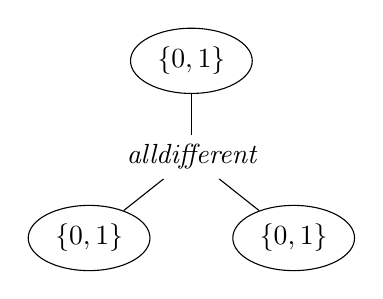
\begin{tikzpicture}
                \node [draw, ellipse] (C1) at (90:1.5) { $\{0,1\}$ };
                \node [draw, ellipse] (C2) at (210:1.5) { $\{0,1\}$ };
                \node [draw, ellipse] (C3) at (330:1.5) {  $\{0,1\}$  };

                \node [anchor = south] (C) at (0, 0) { $\textit{alldifferent}$ };

                \draw (C) to (C1);
                \draw (C) to (C2);
                \draw (C) to (C3);
            \end{tikzpicture}
        \end{column}
    \end{columns}

\end{frame}

\begin{frame}{Decomposing ``All Different''}

    \begin{columns}
        \begin{column}{0.45\textwidth}
            \begin{align*}
                & x_1 \in \{ 0, 1 \} \\
                & x_2 \in \{ 0, 1 \} \\
                & x_3 \in \{ 0, 1 \} \\
                & x_1 \ne x_2 \\
                & x_1 \ne x_3 \\
                & x_2 \ne x_3 \\
            \end{align*}
        \end{column}
        \begin{column}{0.45\textwidth}
            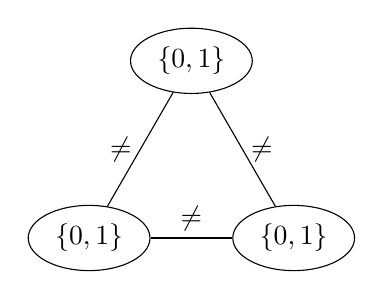
\begin{tikzpicture}
                \node [draw, ellipse] (C1) at (90:1.5) { $\{0,1\}$ };
                \node [draw, ellipse] (C2) at (210:1.5) { $\{0,1\}$ };
                \node [draw, ellipse] (C3) at (330:1.5) {  $\{0,1\}$  };

                \draw (C1) to node [xshift=-0.7em] { $\ne$ } (C2);
                \draw (C1) to node [xshift=0.7em] { $\ne$ } (C3);
                \draw (C2) to node [yshift=0.7em] { $\ne$ } (C3);
            \end{tikzpicture}
        \end{column}
    \end{columns}

\end{frame}

\begin{frame}{What Does Propagation Do?}

    \begin{itemize}
        \item Let's consider the constraint $x_1 \ne x_2$.
            \begin{itemize}
                \item If $x_1 = 0$, we can give $x_2 = 1$, so that's OK.
                \item If $x_1 = 1$, we can give $x_2 = 0$, so that's OK.
                \item If $x_2 = 0$, we can give $x_1 = 1$, so that's OK.
                \item If $x_2 = 1$, we can give $x_1 = 0$, so that's OK.
            \end{itemize}
        \item Let's consider the constraint $x_1 \ne x_3$.
            \begin{itemize}
                \item etc
            \end{itemize}
        \item Let's consider the constraint $x_2 \ne x_3$.
            \begin{itemize}
                \item etc
            \end{itemize}
        \item So no values are deleted, and everything looks OK.
        \item Actually, there's a more efficient algorithm: $\ne$ won't do anything unless one of
            the variables only has one value. Some solvers won't trigger the constraint unless this
            happens.
    \end{itemize}

\end{frame}

\begin{frame}{What Would a Human Do?}
    \begin{center}
        ``Duh, obviously there's no solution! There \\ aren't enough numbers to go around.''
    \end{center}

    \begin{itemize}
        \item Unfortunately ``stare at it for a few seconds then write down the answer'' is not an algorithm.

        \item But if we don't decompose the constraint, we \emph{can} come up with a propagator
            which can tell that there's no solution.
    \end{itemize}
\end{frame}

\begin{frame}{Matchings}

    \begin{columns}
        \begin{column}{0.70\textwidth}
            \begin{itemize}
                \item Draw a vertex on the left for each variable, and a vertex on the right for each value.
                \item Draw edges from each variable to each of its values.
                \item A \emph{maximum cardinality matching} is where you pick as many edges as
                    possible, but each vertex can only be used at most once.
                \item We can find this in polynomial time (see Algorithmics II).
                \item There is a matching which covers each variable if and only if the constraint
                    can be satisfied.
            \end{itemize}
        \end{column}
        \begin{column}{0.28\textwidth}
            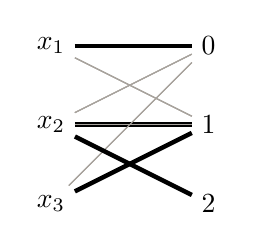
\begin{tikzpicture}
                \node (X1) at (0, 2) { $x_1$ };
                \node (X2) at (0, 1) { $x_2$ };
                \node (X3) at (0, 0) { $x_3$ };

                \node (V0) at (2, 2) { $0$ };
                \node (V1) at (2, 1) { $1$ };
                \node <3-> (V2) at (2, 0) { $2$ };

                \draw <1, 3> [color=uofgsandstone!50] (X1) -- (V0);
                \draw <1, 3> [color=uofgsandstone!50] (X1) -- (V1);
                \draw <1, 3> [color=uofgsandstone!50] (X2) -- (V0);
                \draw <1, 3> [color=uofgsandstone!50] (X2) -- (V1);
                \draw <1, 3> [color=uofgsandstone!50] (X3) -- (V0);
                \draw <1, 3> [color=uofgsandstone!50] (X3) -- (V1);
                \draw <3> [color=uofgsandstone!50] (X2) -- (V2);

                \draw <2> [color=uofgsandstone!50] (X1) -- (V1);
                \draw <2> [color=uofgsandstone!50] (X2) -- (V0);
                \draw <2> [color=uofgsandstone!50] (X3) -- (V0);
                \draw <2> [color=uofgsandstone!50] (X3) -- (V1);
                \draw <2> [ultra thick] (X1) -- (V0);
                \draw <2> [ultra thick] (X2) -- (V1);

                \draw <4> [color=uofgsandstone!50] (X1) -- (V1);
                \draw <4> [color=uofgsandstone!50] (X2) -- (V0);
                \draw <4> [color=uofgsandstone!50] (X2) -- (V1);
                \draw <4> [color=uofgsandstone!50] (X3) -- (V0);
                \draw <4> [ultra thick] (X1) -- (V0);
                \draw <4> [ultra thick] (X3) -- (V1);
                \draw <4> [ultra thick] (X2) -- (V2);
            \end{tikzpicture}
        \end{column}
    \end{columns}

\end{frame}

\begin{frame}{Sudoku}

\end{frame}

\begin{frame}{What Would a Human Do?}
    \begin{center}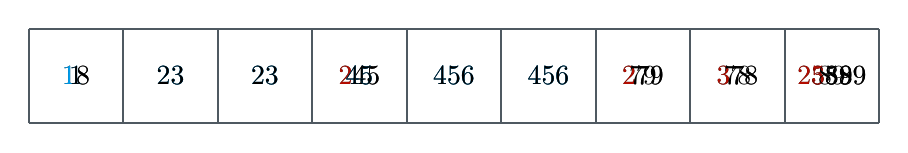
\begin{tikzpicture}[scale=0.4]
        \draw[thick, scale=3, color=uofgslate] (0, 0) grid (9, 1);

        \node <1>   [anchor=center] at (1.5, 1.5)  { 18 };
        \node <2>   [anchor=center] at (1.5, 1.5)  { \textcolor{uofgcobalt}{1}8 };
        \node <3>   [anchor=center] at (1.5, 1.5)  { \textcolor{uofgcobalt}{1} };
        \node <4->  [anchor=center] at (1.5, 1.5)  { 1 };

        \node <1-4> [anchor=center] at (4.5, 1.5)  { 23 };
        \node <5-6> [anchor=center] at (4.5, 1.5)  { \textcolor{uofgcobalt}{23} };
        \node <7->  [anchor=center] at (4.5, 1.5)  { 23 };

        \node <1-4> [anchor=center] at (7.5, 1.5)  { 23 };
        \node <5-6> [anchor=center] at (7.5, 1.5)  { \textcolor{uofgcobalt}{23} };
        \node <7->  [anchor=center] at (7.5, 1.5)  { 23 };

        \node <1-5> [anchor=center] at (10.5, 1.5) { 245 };
        \node <6>   [anchor=center] at (10.5, 1.5) { \textcolor{uofgpillarbox}{2}45 };
        \node <7>   [anchor=center] at (10.5, 1.5) { 45 };
        \node <8-9> [anchor=center] at (10.5, 1.5) { \textcolor{uofgcobalt}{45} };
        \node <10-> [anchor=center] at (10.5, 1.5) { 45 };

        \node <1-7> [anchor=center] at (13.5, 1.5) { 456 };
        \node <8-9>  [anchor=center] at (13.5, 1.5) { \textcolor{uofgcobalt}{456} };
        \node <10-> [anchor=center] at (13.5, 1.5) { 456 };

        \node <1-7> [anchor=center] at (16.5, 1.5) { 456 };
        \node <8-9> [anchor=center] at (16.5, 1.5) { \textcolor{uofgcobalt}{456} };
        \node <10-> [anchor=center] at (16.5, 1.5) { 456 };

        \node <1-5> [anchor=center] at (19.5, 1.5) { 279 };
        \node <6>   [anchor=center] at (19.5, 1.5) { \textcolor{uofgpillarbox}{2}79 };
        \node <7->  [anchor=center] at (19.5, 1.5) { 79 };

        \node <1-5> [anchor=center] at (22.5, 1.5) { 378 };
        \node <6>   [anchor=center] at (22.5, 1.5) { \textcolor{uofgpillarbox}{3}78 };
        \node <7->  [anchor=center] at (22.5, 1.5) { 78 };

        \node <1-5> [anchor=center] at (25.5, 1.5) { 23589 };
        \node <6>   [anchor=center] at (25.5, 1.5) { \textcolor{uofgpillarbox}{23}589 };
        \node <7-8> [anchor=center] at (25.5, 1.5) { 589 };
        \node <9>   [anchor=center] at (25.5, 1.5) { \textcolor{uofgpillarbox}{5}89 };
        \node <10-> [anchor=center] at (25.5, 1.5) { 89 };

    \end{tikzpicture}\end{center}
\end{frame}

\begin{frame}[fragile]{What Does Choco Do?}
    \only<1> {
        \lstinputlisting[language=Java, basicstyle=\scriptsize\ttfamily, keywordstyle=\color{uofgcobalt}]{OneRowSudoku-snippet.java}
    }

    \only<2> {
        \lstinputlisting[basicstyle=\scriptsize\ttfamily]{OneRowSudoku-output.txt}

        \begin{center}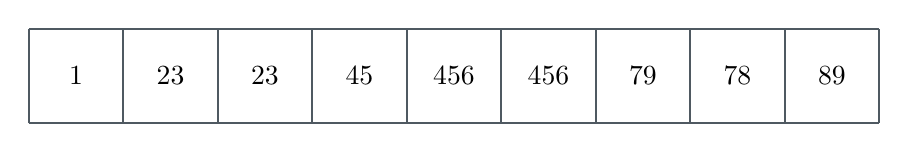
\begin{tikzpicture}[scale=0.4]
            \draw[thick, scale=3, color=uofgslate] (0, 0) grid (9, 1);

            \node [anchor=center] at (1.5, 1.5)  { 1 };
            \node [anchor=center] at (4.5, 1.5)  { 23 };
            \node [anchor=center] at (7.5, 1.5)  { 23 };
            \node [anchor=center] at (10.5, 1.5) { 45 };
            \node [anchor=center] at (13.5, 1.5) { 456 };
            \node [anchor=center] at (16.5, 1.5) { 456 };
            \node [anchor=center] at (19.5, 1.5) { 79 };
            \node [anchor=center] at (22.5, 1.5) { 78 };
            \node [anchor=center] at (25.5, 1.5) { 89 };

        \end{tikzpicture}\end{center}
    }

    \only<3> {
        \lstinputlisting[language=Java, basicstyle=\scriptsize\ttfamily, keywordstyle=\color{uofgcobalt}]{OneRowSudoku-neq-snippet.java}
    }

    \only<4> {
        \lstinputlisting[basicstyle=\scriptsize\ttfamily]{OneRowSudoku-neq-output.txt}
    }
\end{frame}

\begin{frame}{Matchings, Again}
    \centering
    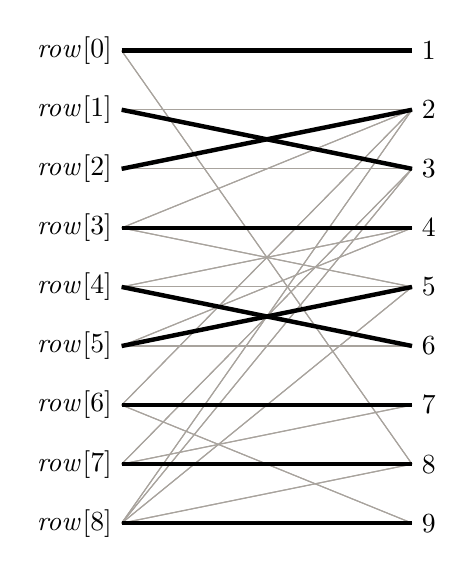
\begin{tikzpicture}[scale=0.75]
        \node <2-> (X1) at (0, 8) { $\mathit{row}[0]$ };
        \node <2-> (X2) at (0, 7) { $\mathit{row}[1]$ };
        \node <2-> (X3) at (0, 6) { $\mathit{row}[2]$ };
        \node <2-> (X4) at (0, 5) { $\mathit{row}[3]$ };
        \node <2-> (X5) at (0, 4) { $\mathit{row}[4]$ };
        \node <2-> (X6) at (0, 3) { $\mathit{row}[5]$ };
        \node <2-> (X7) at (0, 2) { $\mathit{row}[6]$ };
        \node <2-> (X8) at (0, 1) { $\mathit{row}[7]$ };
        \node <2-> (X9) at (0, 0) { $\mathit{row}[8]$ };

        \node <1-2> (V1) at (6, 8) { $\phantom{1}$ };
        \node <3-> (V1) at (6, 8) { $1$ };
        \node <3-> (V2) at (6, 7) { $2$ };
        \node <3-> (V3) at (6, 6) { $3$ };
        \node <3-> (V4) at (6, 5) { $4$ };
        \node <3-> (V5) at (6, 4) { $5$ };
        \node <3-> (V6) at (6, 3) { $6$ };
        \node <3-> (V7) at (6, 2) { $7$ };
        \node <3-> (V8) at (6, 1) { $8$ };
        \node <3-> (V9) at (6, 0) { $9$ };

        \draw <4> [color=uofgsandstone!50] (X1.east) -- (V1.west);
        \draw <4> [color=uofgsandstone!50] (X1.east) -- (V8.west);
        \draw <4> [color=uofgsandstone!50] (X2.east) -- (V2.west);
        \draw <4> [color=uofgsandstone!50] (X2.east) -- (V3.west);
        \draw <4> [color=uofgsandstone!50] (X3.east) -- (V2.west);
        \draw <4> [color=uofgsandstone!50] (X3.east) -- (V3.west);
        \draw <4> [color=uofgsandstone!50] (X4.east) -- (V2.west);
        \draw <4> [color=uofgsandstone!50] (X4.east) -- (V4.west);
        \draw <4> [color=uofgsandstone!50] (X4.east) -- (V5.west);
        \draw <4> [color=uofgsandstone!50] (X5.east) -- (V4.west);
        \draw <4> [color=uofgsandstone!50] (X5.east) -- (V5.west);
        \draw <4> [color=uofgsandstone!50] (X5.east) -- (V6.west);
        \draw <4> [color=uofgsandstone!50] (X6.east) -- (V4.west);
        \draw <4> [color=uofgsandstone!50] (X6.east) -- (V5.west);
        \draw <4> [color=uofgsandstone!50] (X6.east) -- (V6.west);
        \draw <4> [color=uofgsandstone!50] (X7.east) -- (V2.west);
        \draw <4> [color=uofgsandstone!50] (X7.east) -- (V7.west);
        \draw <4> [color=uofgsandstone!50] (X7.east) -- (V9.west);
        \draw <4> [color=uofgsandstone!50] (X8.east) -- (V3.west);
        \draw <4> [color=uofgsandstone!50] (X8.east) -- (V7.west);
        \draw <4> [color=uofgsandstone!50] (X8.east) -- (V8.west);
        \draw <4> [color=uofgsandstone!50] (X9.east) -- (V2.west);
        \draw <4> [color=uofgsandstone!50] (X9.east) -- (V3.west);
        \draw <4> [color=uofgsandstone!50] (X9.east) -- (V5.west);
        \draw <4> [color=uofgsandstone!50] (X9.east) -- (V8.west);
        \draw <4> [color=uofgsandstone!50] (X9.east) -- (V9.west);

        \draw <5> [color=uofgsandstone!50] (X1.east) -- (V8.west);
        \draw <5> [color=uofgsandstone!50] (X2.east) -- (V2.west);
        \draw <5> [color=uofgsandstone!50] (X3.east) -- (V3.west);
        \draw <5> [color=uofgsandstone!50] (X4.east) -- (V2.west);
        \draw <5> [color=uofgsandstone!50] (X4.east) -- (V5.west);
        \draw <5> [color=uofgsandstone!50] (X5.east) -- (V4.west);
        \draw <5> [color=uofgsandstone!50] (X5.east) -- (V5.west);
        \draw <5> [color=uofgsandstone!50] (X6.east) -- (V4.west);
        \draw <5> [color=uofgsandstone!50] (X6.east) -- (V6.west);
        \draw <5> [color=uofgsandstone!50] (X7.east) -- (V2.west);
        \draw <5> [color=uofgsandstone!50] (X7.east) -- (V9.west);
        \draw <5> [color=uofgsandstone!50] (X8.east) -- (V3.west);
        \draw <5> [color=uofgsandstone!50] (X8.east) -- (V7.west);
        \draw <5> [color=uofgsandstone!50] (X9.east) -- (V2.west);
        \draw <5> [color=uofgsandstone!50] (X9.east) -- (V3.west);
        \draw <5> [color=uofgsandstone!50] (X9.east) -- (V5.west);
        \draw <5> [color=uofgsandstone!50] (X9.east) -- (V8.west);
        \draw <5> [ultra thick] (X9.east) -- (V9.west);
        \draw <5> [ultra thick] (X1.east) -- (V1.west);
        \draw <5> [ultra thick] (X2.east) -- (V3.west);
        \draw <5> [ultra thick] (X3.east) -- (V2.west);
        \draw <5> [ultra thick] (X4.east) -- (V4.west);
        \draw <5> [ultra thick] (X5.east) -- (V6.west);
        \draw <5> [ultra thick] (X6.east) -- (V5.west);
        \draw <5> [ultra thick] (X7.east) -- (V7.west);
        \draw <5> [ultra thick] (X8.east) -- (V8.west);
    \end{tikzpicture}

\end{frame}

\begin{frame}{Hall Sets}
    \begin{itemize}
        \item A \emph{Hall set} of size $n$ is a set of $n$ variables from an ``all different''
            constraint, whose domains have $n$ values between them.

        \item If we can find a Hall set, we can safely remove these values from the domains of every
            other variable involved in the constraint.

        \item If we do this for every Hall set, we delete every value that cannot appear in at least
            one way of satisfying the constraint.
    \end{itemize}
\end{frame}

\begin{frame}{A Magic Trick}

    \only<1> {
        \begin{itemize}
            \item Even though there are $2^n$ potential Hall sets, we can do this in polynomial time using matching
                algorithms.

            \item This algorithm isn't examinable, but here's an animation of roughly how it works, so you don't have to
                believe it's magic any more.
        \end{itemize}
    }

    \only <2-> {
        \centering
        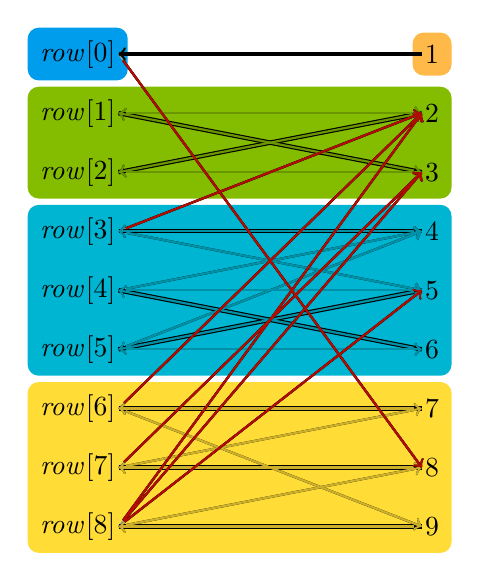
\begin{tikzpicture}[scale=0.75]
            \node [inner sep=1pt] (X1) at (0, 8) { $\mathit{row}[0]$ };
            \node [inner sep=1pt] (X2) at (0, 7) { $\mathit{row}[1]$ };
            \node [inner sep=1pt] (X3) at (0, 6) { $\mathit{row}[2]$ };
            \node [inner sep=1pt] (X4) at (0, 5) { $\mathit{row}[3]$ };
            \node [inner sep=1pt] (X5) at (0, 4) { $\mathit{row}[4]$ };
            \node [inner sep=1pt] (X6) at (0, 3) { $\mathit{row}[5]$ };
            \node [inner sep=1pt] (X7) at (0, 2) { $\mathit{row}[6]$ };
            \node [inner sep=1pt] (X8) at (0, 1) { $\mathit{row}[7]$ };
            \node [inner sep=1pt] (X9) at (0, 0) { $\mathit{row}[8]$ };

            \node [inner sep=1pt] (V1) at (6, 8) { $1$ };
            \node [inner sep=1pt] (V2) at (6, 7) { $2$ };
            \node [inner sep=1pt] (V3) at (6, 6) { $3$ };
            \node [inner sep=1pt] (V4) at (6, 5) { $4$ };
            \node [inner sep=1pt] (V5) at (6, 4) { $5$ };
            \node [inner sep=1pt] (V6) at (6, 3) { $6$ };
            \node [inner sep=1pt] (V7) at (6, 2) { $7$ };
            \node [inner sep=1pt] (V8) at (6, 1) { $8$ };
            \node [inner sep=1pt] (V9) at (6, 0) { $9$ };

            \draw <2> [color=uofgsandstone!50] (X1.east) -- (V8.west);
            \draw <2> [color=uofgsandstone!50] (X2.east) -- (V2.west);
            \draw <2> [color=uofgsandstone!50] (X3.east) -- (V3.west);
            \draw <2> [color=uofgsandstone!50] (X4.east) -- (V2.west);
            \draw <2> [color=uofgsandstone!50] (X4.east) -- (V5.west);
            \draw <2> [color=uofgsandstone!50] (X5.east) -- (V4.west);
            \draw <2> [color=uofgsandstone!50] (X5.east) -- (V5.west);
            \draw <2> [color=uofgsandstone!50] (X6.east) -- (V4.west);
            \draw <2> [color=uofgsandstone!50] (X6.east) -- (V6.west);
            \draw <2> [color=uofgsandstone!50] (X7.east) -- (V2.west);
            \draw <2> [color=uofgsandstone!50] (X7.east) -- (V9.west);
            \draw <2> [color=uofgsandstone!50] (X8.east) -- (V3.west);
            \draw <2> [color=uofgsandstone!50] (X8.east) -- (V7.west);
            \draw <2> [color=uofgsandstone!50] (X9.east) -- (V2.west);
            \draw <2> [color=uofgsandstone!50] (X9.east) -- (V3.west);
            \draw <2> [color=uofgsandstone!50] (X9.east) -- (V5.west);
            \draw <2> [color=uofgsandstone!50] (X9.east) -- (V8.west);
            \draw <2> [color=uofgsandstone!50] (X9.east) -- (V9.west);
            \draw <2> [ultra thick] (X1.east) -- (V1.west);
            \draw <2> [ultra thick] (X2.east) -- (V3.west);
            \draw <2> [ultra thick] (X3.east) -- (V2.west);
            \draw <2> [ultra thick] (X4.east) -- (V4.west);
            \draw <2> [ultra thick] (X5.east) -- (V6.west);
            \draw <2> [ultra thick] (X6.east) -- (V5.west);
            \draw <2> [ultra thick] (X7.east) -- (V7.west);
            \draw <2> [ultra thick] (X8.east) -- (V8.west);
            \draw <2> [ultra thick] (X9.east) -- (V9.west);

            \draw <3-4> [thick, ->, shorten <=0.1cm] (X1.east) -- (V8.west);
            \draw <3-4> [thick, ->, shorten <=0.1cm] (X2.east) -- (V2.west);
            \draw <3-4> [thick, ->, shorten <=0.1cm] (X3.east) -- (V3.west);
            \draw <3-4> [thick, ->, shorten <=0.1cm] (X4.east) -- (V2.west);
            \draw <3-4> [thick, ->, shorten <=0.1cm] (X4.east) -- (V5.west);
            \draw <3-4> [thick, ->, shorten <=0.1cm] (X5.east) -- (V4.west);
            \draw <3-4> [thick, ->, shorten <=0.1cm] (X5.east) -- (V5.west);
            \draw <3-4> [thick, ->, shorten <=0.1cm] (X6.east) -- (V4.west);
            \draw <3-4> [thick, ->, shorten <=0.1cm] (X6.east) -- (V6.west);
            \draw <3-4> [thick, ->, shorten <=0.1cm] (X7.east) -- (V2.west);
            \draw <3-4> [thick, ->, shorten <=0.1cm] (X7.east) -- (V9.west);
            \draw <3-4> [thick, ->, shorten <=0.1cm] (X8.east) -- (V3.west);
            \draw <3-4> [thick, ->, shorten <=0.1cm] (X8.east) -- (V7.west);
            \draw <3-4> [thick, ->, shorten <=0.1cm] (X9.east) -- (V2.west);
            \draw <3-4> [thick, ->, shorten <=0.1cm] (X9.east) -- (V3.west);
            \draw <3-4> [thick, ->, shorten <=0.1cm] (X9.east) -- (V5.west);
            \draw <3-4> [thick, ->, shorten <=0.1cm] (X9.east) -- (V8.west);
            \draw <3-4> [thick, <-, shorten >=0.1cm] (X9.east) -- (V9.west);
            \draw <3-4> [thick, <-, shorten >=0.1cm] (X1.east) -- (V1.west);
            \draw <3-4> [thick, <-, shorten >=0.1cm] (X2.east) -- (V3.west);
            \draw <3-4> [thick, <-, shorten >=0.1cm] (X3.east) -- (V2.west);
            \draw <3-4> [thick, <-, shorten >=0.1cm] (X4.east) -- (V4.west);
            \draw <3-4> [thick, <-, shorten >=0.1cm] (X5.east) -- (V6.west);
            \draw <3-4> [thick, <-, shorten >=0.1cm] (X6.east) -- (V5.west);
            \draw <3-4> [thick, <-, shorten >=0.1cm] (X7.east) -- (V7.west);
            \draw <3-4> [thick, <-, shorten >=0.1cm] (X8.east) -- (V8.west);

            \draw <5> [thick, ->, shorten <=0.1cm, color=uofglawn!80!black] (X2.east) -- (V2.west);
            \draw <5> [thick, ->, shorten <=0.1cm, color=uofglawn!80!black] (X3.east) -- (V3.west);
            \draw <5> [thick, <-, shorten >=0.1cm, color=uofglawn!80!black] (X2.east) -- (V3.west);
            \draw <5> [thick, <-, shorten >=0.1cm, color=uofglawn!80!black] (X3.east) -- (V2.west);
            \draw <5> [thick, ->, shorten <=0.1cm, color=uofgturquoise!80!black] (X4.east) -- (V5.west);
            \draw <5> [thick, ->, shorten <=0.1cm, color=uofgturquoise!80!black] (X5.east) -- (V4.west);
            \draw <5> [thick, ->, shorten <=0.1cm, color=uofgturquoise!80!black] (X5.east) -- (V5.west);
            \draw <5> [thick, ->, shorten <=0.1cm, color=uofgturquoise!80!black] (X6.east) -- (V4.west);
            \draw <5> [thick, ->, shorten <=0.1cm, color=uofgturquoise!80!black] (X6.east) -- (V6.west);
            \draw <5> [thick, <-, shorten >=0.1cm, color=uofgturquoise!80!black] (X4.east) -- (V4.west);
            \draw <5> [thick, <-, shorten >=0.1cm, color=uofgturquoise!80!black] (X5.east) -- (V6.west);
            \draw <5> [thick, <-, shorten >=0.1cm, color=uofgturquoise!80!black] (X6.east) -- (V5.west);
            \draw <5> [thick, ->, shorten <=0.1cm, color=uofgsunshine!80!black] (X7.east) -- (V9.west);
            \draw <5> [thick, ->, shorten <=0.1cm, color=uofgsunshine!80!black] (X8.east) -- (V7.west);
            \draw <5> [thick, ->, shorten <=0.1cm, color=uofgsunshine!80!black] (X9.east) -- (V8.west);
            \draw <5> [thick, <-, shorten >=0.1cm, color=uofgsunshine!80!black] (X9.east) -- (V9.west);
            \draw <5> [thick, <-, shorten >=0.1cm, color=uofgsunshine!80!black] (X7.east) -- (V7.west);
            \draw <5> [thick, <-, shorten >=0.1cm, color=uofgsunshine!80!black] (X8.east) -- (V8.west);
            \draw <7-> [thick, <-, shorten >=0.1cm, color=uofglawn] (X1.east) -- (V1.west);
            \draw <5-6>  [thick, <-, shorten >=0.1cm] (X1.east) -- (V1.west);
            \draw <5-6>  [thick, ->, shorten <=0.1cm] (X4.east) -- (V2.west);
            \draw <5-6>  [thick, ->, shorten <=0.1cm] (X7.east) -- (V2.west);
            \draw <5-6>  [thick, ->, shorten <=0.1cm] (X8.east) -- (V3.west);
            \draw <5-6>  [thick, ->, shorten <=0.1cm] (X9.east) -- (V2.west);
            \draw <5-6>  [thick, ->, shorten <=0.1cm] (X9.east) -- (V3.west);
            \draw <5-6>  [thick, ->, shorten <=0.1cm] (X9.east) -- (V5.west);
            \draw <5-6>  [thick, ->, shorten <=0.1cm] (X1.east) -- (V8.west);
            \draw <7->  [thick, ->, shorten <=0.1cm, color=uofgpillarbox] (X4.east) -- (V2.west);
            \draw <7->  [thick, ->, shorten <=0.1cm, color=uofgpillarbox] (X7.east) -- (V2.west);
            \draw <7->  [thick, ->, shorten <=0.1cm, color=uofgpillarbox] (X8.east) -- (V3.west);
            \draw <7->  [thick, ->, shorten <=0.1cm, color=uofgpillarbox] (X9.east) -- (V2.west);
            \draw <7->  [thick, ->, shorten <=0.1cm, color=uofgpillarbox] (X9.east) -- (V3.west);
            \draw <7->  [thick, ->, shorten <=0.1cm, color=uofgpillarbox] (X9.east) -- (V5.west);
            \draw <7->  [thick, ->, shorten <=0.1cm, color=uofgpillarbox] (X1.east) -- (V8.west);

            \begin{pgfonlayer}{background}
                \node [rounded corners, fit = (X1)] {};
                \node [rounded corners, fit = (V1)] {};
                \node [rounded corners, fit = (X2) (X3) (V2) (V3)] {};
                \node [rounded corners, fit = (X4) (X5) (X6) (V4) (V5) (V6)] {};
                \node [rounded corners, fit = (X7) (X8) (X9) (V7) (V8) (V9)] {};
                \node <4-5> [rounded corners, fit = (X1), fill=uofgcobalt] {};
                \node <4-5> [rounded corners, fit = (V1), fill=uofgpumpkin] {};
                \node <4-5> [rounded corners, fit = (X2) (X3) (V2) (V3), fill=uofglawn] {};
                \node <4-5> [rounded corners, fit = (X4) (X5) (X6) (V4) (V5) (V6), fill=uofgturquoise] {};
                \node <4-5> [rounded corners, fit = (X7) (X8) (X9) (V7) (V8) (V9), fill=uofgsunshine] {};
            \end{pgfonlayer}
        \end{tikzpicture}
    }
\end{frame}

\begin{frame}{Only Occurs in One Place?}

    \begin{center}
        ``But wait! We said that the value 1 only occurs \\
        in one place. That doesn't sound like a Hall set!''
    \end{center}

    \begin{itemize}
        \item <2-> The ``only occurs in one place'' rule we used first is just a Hall set of size 8.
    \end{itemize}
\end{frame}

\begin{frame}[fragile]{A Sudoku Solver in Choco}
    \only<1>{\lstinputlisting[language=Java, basicstyle=\scriptsize\ttfamily, keywordstyle=\color{uofgcobalt}]{Sudoku-1-snippet.java}}
    \only<2>{\lstinputlisting[language=Java, basicstyle=\scriptsize\ttfamily, keywordstyle=\color{uofgcobalt}]{Sudoku-2-snippet.java}}
    \only<3>{\lstinputlisting[language=Java, basicstyle=\scriptsize\ttfamily, keywordstyle=\color{uofgcobalt}]{Sudoku-3-snippet.java}}
    \only<4>{\lstinputlisting[language=Java, basicstyle=\scriptsize\ttfamily, keywordstyle=\color{uofgcobalt}]{Sudoku-4-snippet.java}}
    \only<5>{\lstinputlisting[language=Java, basicstyle=\scriptsize\ttfamily, keywordstyle=\color{uofgcobalt}]{Sudoku-5-snippet.java}}
    \only<6>{\lstinputlisting[language=Java, basicstyle=\scriptsize\ttfamily, keywordstyle=\color{uofgcobalt}]{Sudoku-6-snippet.java}}
    \only<7>{\lstinputlisting[language=Java, basicstyle=\scriptsize\ttfamily, keywordstyle=\color{uofgcobalt}]{Sudoku-7-snippet.java}}
\end{frame}

\begin{frame}[fragile]{Incidentally, 2D arrays in Gecode are Much Nicer}
    \lstinputlisting[language=C++, basicstyle=\scriptsize\ttfamily, keywordstyle=\color{uofgcobalt}]{GecodeSudoku-snippet.cc}
\end{frame}

\begin{frame}{Some Experiments}
    \only<1> {
        \lstinputlisting[basicstyle=\scriptsize\ttfamily]{herald20061222E.txt}
    }
    \only<2-3> {
        \begin{columns}
            \begin{column}{0.45\textwidth}
                \lstinputlisting[basicstyle=\scriptsize\ttfamily]{herald20061222E-neq.txt}
            \end{column}
            \begin{column}{0.45\textwidth}
                \only<3>{
                    \lstinputlisting[basicstyle=\scriptsize\ttfamily]{herald20061222E-alldiff.txt}
                }
            \end{column}
        \end{columns}
    }

    \only<4> {
        \lstinputlisting[basicstyle=\scriptsize\ttfamily]{herald20061222H.txt}
    }
    \only<5-6> {
        \begin{columns}
            \begin{column}{0.45\textwidth}
                \lstinputlisting[basicstyle=\scriptsize\ttfamily]{herald20061222H-neq.txt}
            \end{column}
            \begin{column}{0.45\textwidth}
                \only<6>{
                    \lstinputlisting[basicstyle=\scriptsize\ttfamily]{herald20061222H-alldiff.txt}
                }
            \end{column}
        \end{columns}
    }

    \only<7> {
        \lstinputlisting[basicstyle=\scriptsize\ttfamily]{times20070107.txt}
    }
    \only<8-9> {
        \begin{columns}
            \begin{column}{0.45\textwidth}
                \lstinputlisting[basicstyle=\scriptsize\ttfamily]{times20070107-neq.txt}
            \end{column}
            \begin{column}{0.45\textwidth}
                \only<9>{
                    \lstinputlisting[basicstyle=\scriptsize\ttfamily]{times20070107-alldiff.txt}
                }
            \end{column}
        \end{columns}
    }

    \only<10> {
        \includegraphics*[keepaspectratio=true,scale=0.24]{hardest.png}
    }
    \only<11-12> {
        \begin{columns}
            \begin{column}{0.45\textwidth}
                \lstinputlisting[basicstyle=\scriptsize\ttfamily]{hardest-neq.txt}
            \end{column}
            \begin{column}{0.45\textwidth}
                \only<12>{
                    \lstinputlisting[basicstyle=\scriptsize\ttfamily]{hardest-alldiff.txt}
                }
            \end{column}
        \end{columns}
    }
\end{frame}

\begin{frame}{Do Global Constraints Always Help?}
    \begin{itemize}
        \item Sometimes globals make a spectacular difference.

        \item Sometimes global constraints end up not giving any more deletions than their
            decompositions, and can take longer to propagate.

        \item Sometimes extra deletions don't reduce the search space size.

        \item Using globals isn't a \emph{guaranteed} benefit, but they make the model easier to
            read, and it's easier to translate from globals to decompositions than the other way
            around.
    \end{itemize}
\end{frame}

\begin{frame}{Some Other Interesting Global Constraints}

    \begin{itemize}
        \item All different except 0.
        \item Global cardinality.
        \item At least, at most, among.
        \item $n$ Value.
        \item Regular.
    \end{itemize}

\end{frame}

\begin{frame}{Are You Smarter than a Constraint Solver?}
    \only<1> {
        \begin{center}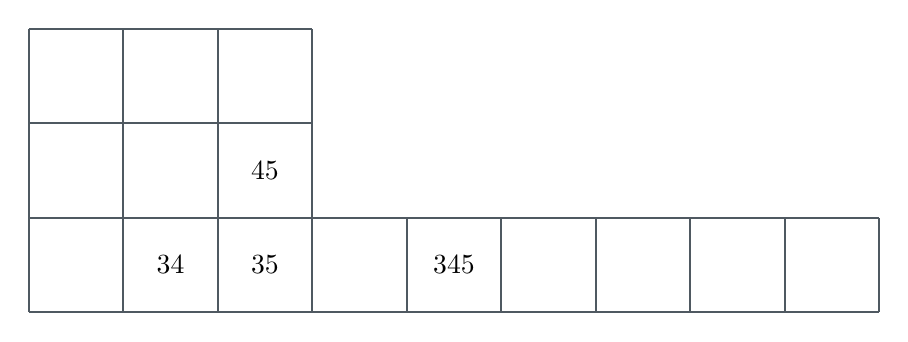
\begin{tikzpicture}[scale=0.4]
            \draw[thick, scale=3, color=uofgslate] (0, 0) grid (3, 3);
            \draw[thick, scale=3, color=uofgslate] (3, 0) grid (9, 1);

            \node[anchor=center] at (4.5, 1.5) { 34 };
            \node[anchor=center] at (7.5, 1.5) { 35 };
            \node[anchor=center] at (7.5, 4.5) { 45 };
            \node[anchor=center] at (13.5, 1.5) { 345 };

        \end{tikzpicture}\end{center}
    }

    \only<2> {
        \begin{itemize}
            \item Remember: propagation only considers \emph{one constraint at a time}, and the only
                communication between constraints is by deleting values.

            \item Automatically combining certain constraints is an active research topic.
                \begin{itemize}
                    \item But getting ``the best possible'' filtering from two ``all different''
                        constraints simultaneously is \NP-hard\ldots
                \end{itemize}
        \end{itemize}
    }
\end{frame}

\begin{frame}{This is Not The Exam Question}

    What is a \emph{Hall set}, and why is it useful for propagation? Use the following model to
    illustrate your answer:
    \begin{align*}
        & x_1 \in \{ 4, 5 \}   && x_2 \in \{ 1, 2, 3, 4 \}  && x_3 \in \{ 3, 4, 5 \} \\
        & x_4 \in \{ 5, 6 \}   && x_5 \in \{ 3, 5 \} \\
        & \mathrlap{\textit{alldifferent}( x_1, x_2, x_3, x_4, x_5 )}
    \end{align*}

    Suppose our solver did not have an ``all different'' constraint. Show how to rewrite this model
    using only binary constraints.  What effect would this have on propagation? \\[0.2cm]

    Aside from propagation, describe another benefit of global constraints.

\end{frame}

\begin{frame}[plain,noframenumbering]
    \begin{tikzpicture}[remember picture, overlay]
        \node at (current page.north west) {
            \begin{tikzpicture}[remember picture, overlay]
                \fill [fill=uofguniversityblue, anchor=north west] (0, 0) rectangle (\paperwidth, -1.7cm);
            \end{tikzpicture}
        };

        \node (logo) [anchor=north east, shift={(-0.3cm,-0.2cm)}] at (current page.north east) {
            \includegraphics*[keepaspectratio=true,scale=0.55]{UoG_keyline.pdf}
        };
    \end{tikzpicture}
\end{frame}

\end{document}


